\chapter{Optimization Results}
\label{sec:optimization_results}
This chapter focuses on showing and analyzing the most interesting MAV designs
outputted by the optimization tool. A short digression on platonic solid is first
needed to properly analyse the results. The optimal designs with an even number
of propellers are then described. Afterwards, the designs with an odd number of
propellers are shown. A comparison of the different optimal drone design is then
proposed. Finally, a few results of optimizations performed with the number of
propeller as an argument are presented.

\section{Platonic Solids}
\label{sec:platonic_solids}
Platonic solids are five regular and convex polyhedrons named after the
ancient Greek philosopher Plato to honor his memory \citep{noauthor_platonic_2018}.
The five platonic solids are:
\begin{itemize}
\item The tetrahedron composed of four faces and four vertices (see \Cref{fig:tetrahedron}).
\item The octahedron composed of eight faces and six vertices (see \Cref{fig:octahedron}).
\item The cube composed of six faces and eight vertices (see \Cref{fig:cube}).
\item The icosahedron composed of twenty faces and twelve vertices.
\item The dodecahedron composed of twelve faces and twenty vertices.
\end{itemize}
There is a angle that can be found at least in the
first three platonic solids. This angle is found between the horizontal plane and
the vertices of the polyhedron (see \Cref{fig:platonic_solid}). To ensure simplicity,
in the rest of this work this angle will be referred to as the platonic solids angle
and $\beta_{PS}$).

\begin{figure}[!h]
  \begin{subfigure}[b]{0.22\textwidth}
    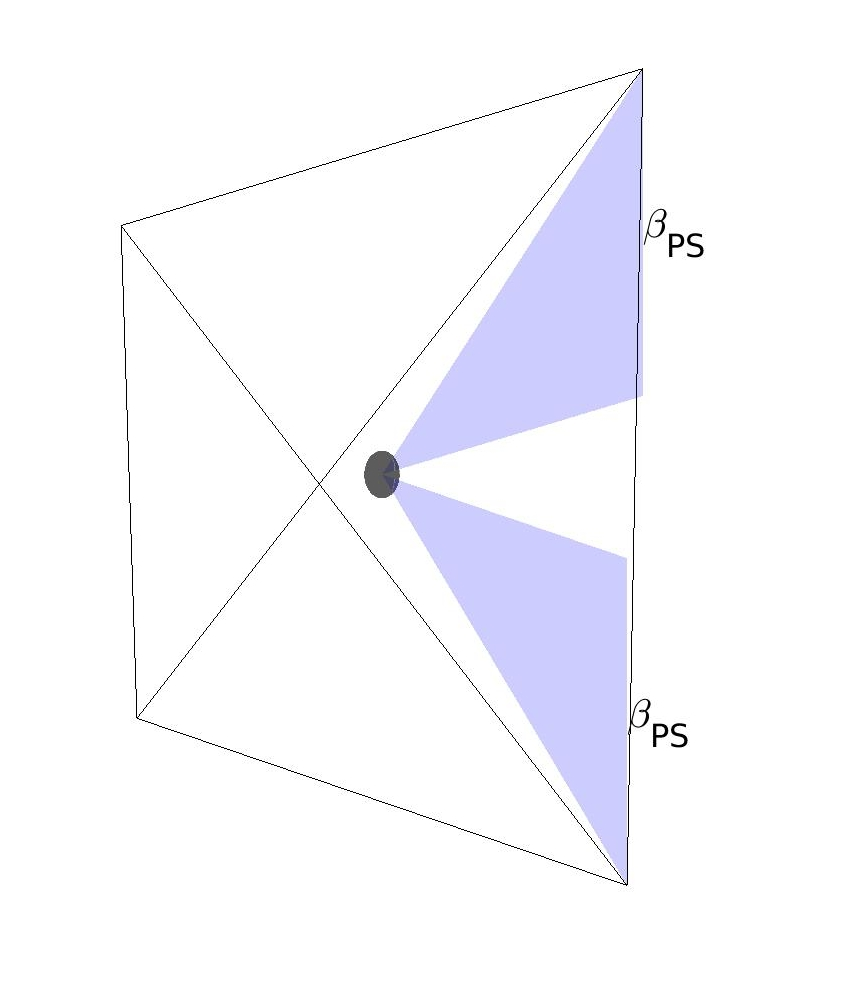
\includegraphics[width=\linewidth]{images/tetrahedron.jpg}
    \caption{Tetrahedron.} \label{fig:tetrahedron}
  \end{subfigure}
  \hspace*{\fill} % separation between the subfigures
  \begin{subfigure}[b]{0.27\textwidth}
    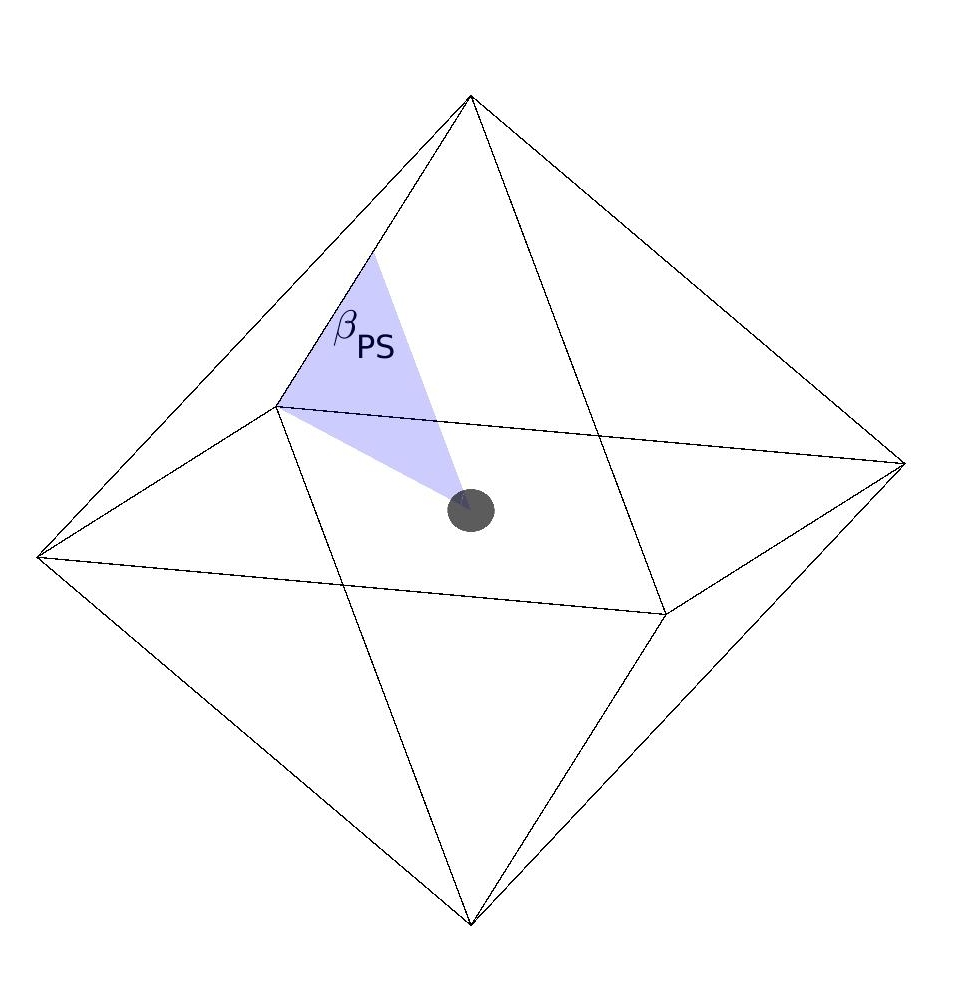
\includegraphics[width=\linewidth]{images/octahedron.jpg}
    \caption{Octahedron.} \label{fig:octahedron}
  \end{subfigure}
  \hspace*{\fill} % separation between the subfigures
  \begin{subfigure}[b]{0.26\textwidth}
    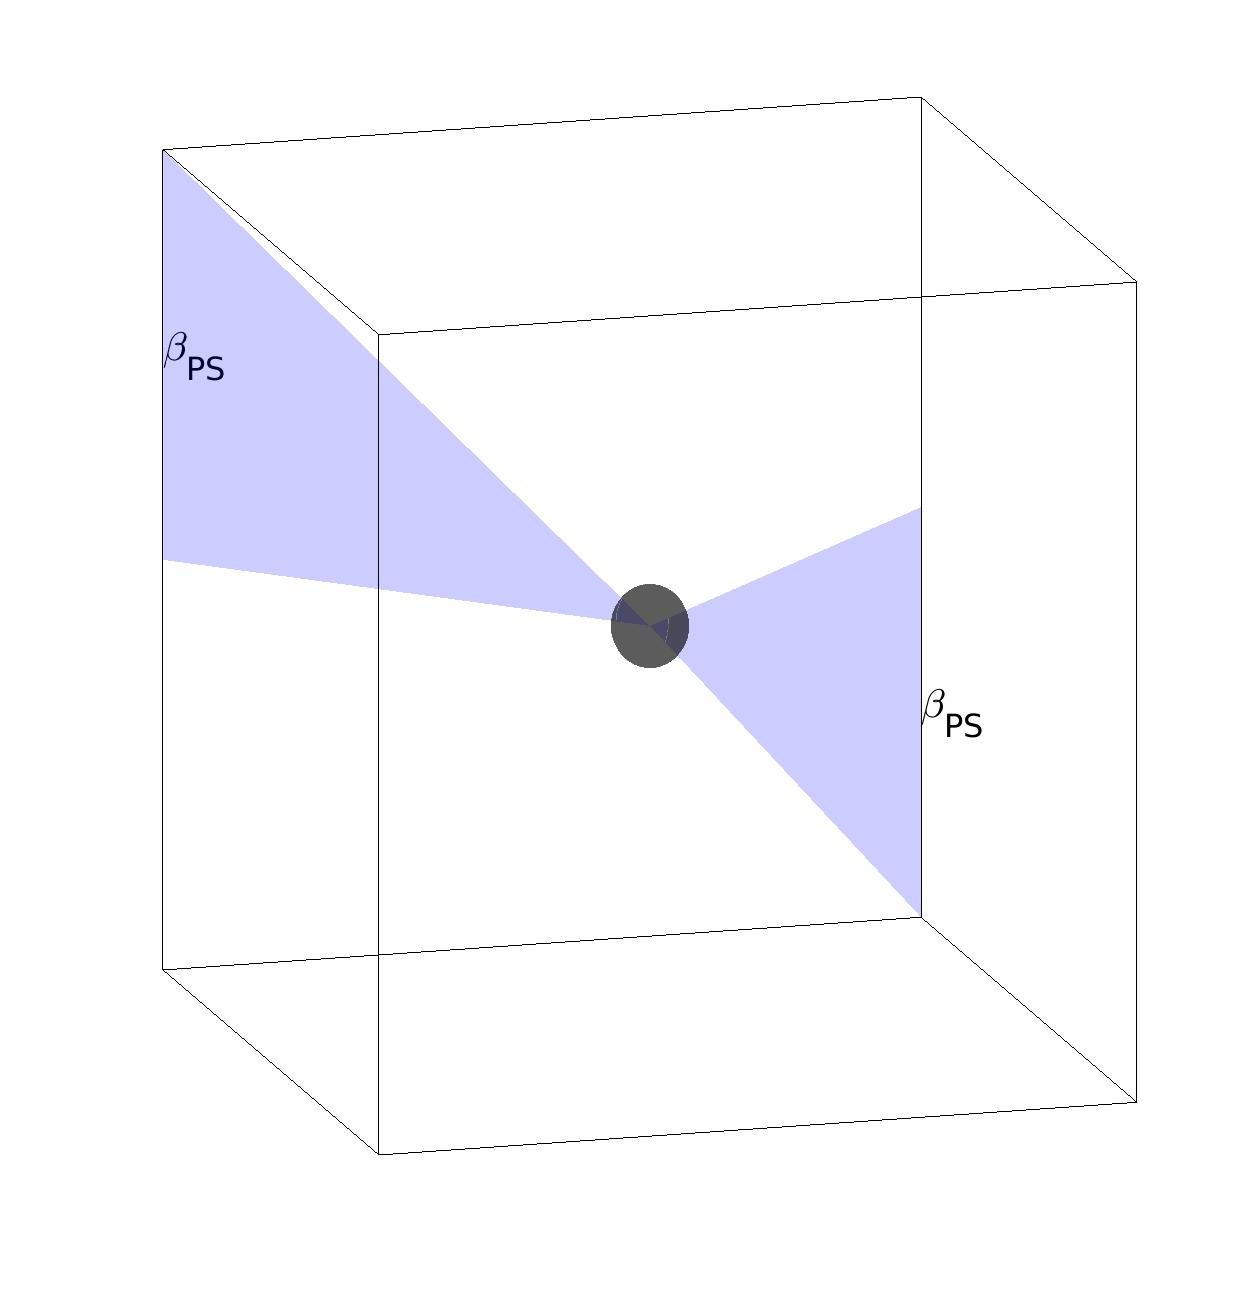
\includegraphics[width=\linewidth]{images/cube.jpg}
    \caption{Cube.} \label{fig:cube}
  \end{subfigure}
  \caption{The first three platonic solids $\big(\cos(\beta_{PS}) = \sqrt{\frac{2}{3}}
  =>  \beta_{PS} \simeq 35.26^{\circ}\big)\, .$}
  \label{fig:platonic_solid}
\end{figure}



\section{Even Designs}
\label{sec:even_designs}

\subsection{Quad-copter}
\label{sec:quad_copter}
Design 1:
\begin{itemize}
  \item $n\ =\ 4$
  \item $\beta_{arm}\ =\ [35.26^{\circ},\  -35.26^{\circ},\  35.26^{\circ},\  -35.26^{\circ}]$
  \item $\theta_{arm}\ =\ [0^{\circ},\  0^{\circ},\  0^{\circ},\  0^{\circ}]$
  \item $L\ =\ 0.5\ [m]$
\end{itemize}

Design 2:
\begin{itemize}
  \item $n\ =\ 4$
  \item $\beta_{arm}\ =\ [-32.42^{\circ},\  -35.49^{\circ},\  -35.44^{\circ},\  -35.49^{\circ}]$
  \item $\theta_{arm}\ =\ [-0.99^{\circ},\  -1.88^{\circ},\  -2.26^{\circ},\  -2.94^{\circ}]$
  \item $L\ =\ 0.5\ [m]$
\end{itemize}


\begin{figure}[!h]
  \resizebox{\textwidth}{!}{\begin{subfigure}[b]{0.4\textwidth}
    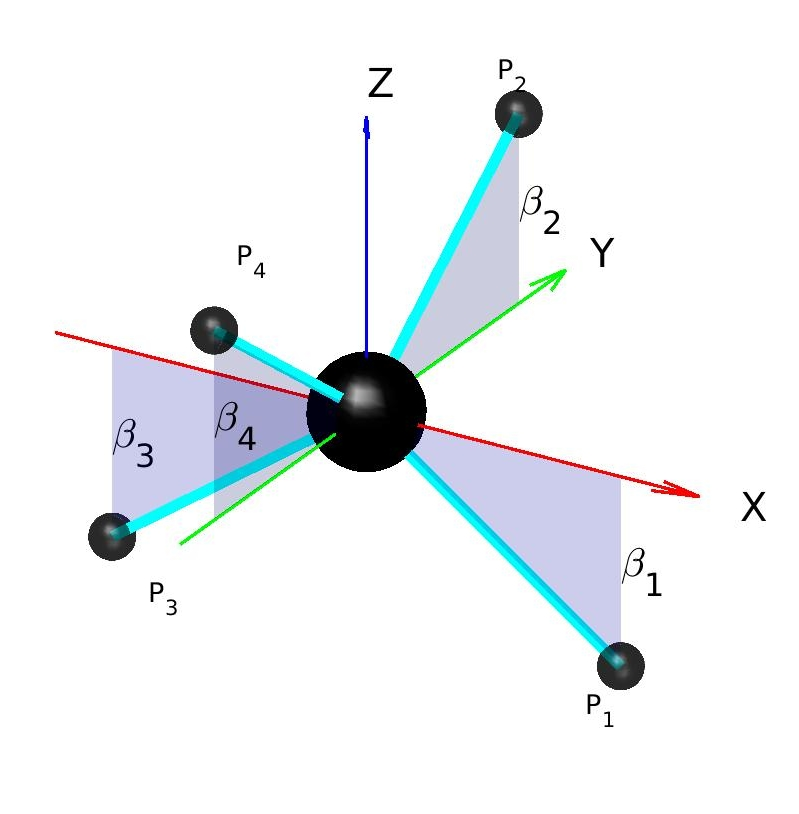
\includegraphics[width=\linewidth]{images/Quadcopter.jpg}
    \caption{Optimal quad-copter design 1} \label{fig:Quadcopter_resulta}
  \end{subfigure}
  \hspace*{\fill} % separation between the subfigures
  \begin{subfigure}[b]{0.35\textwidth}
    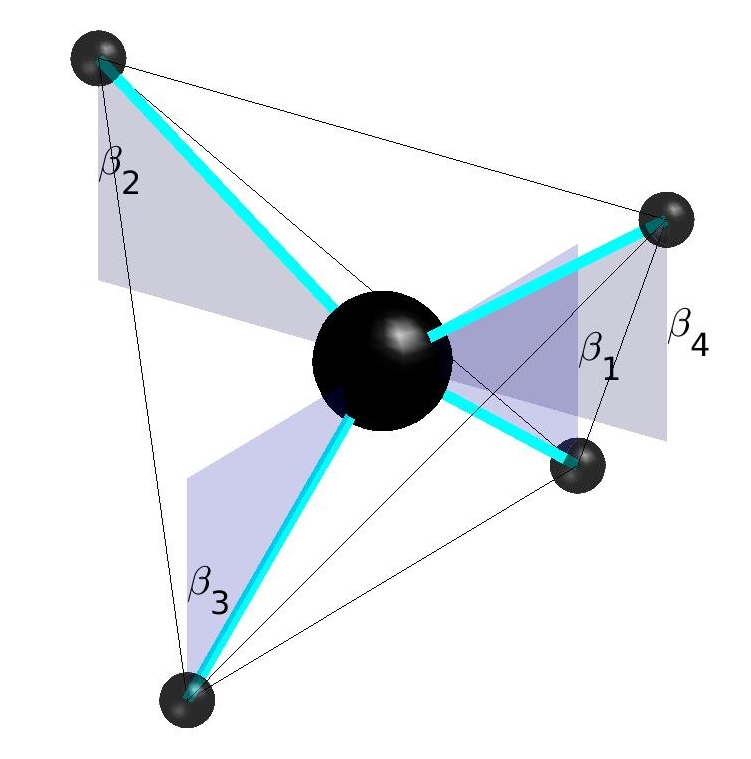
\includegraphics[width=\linewidth]{images/Quad_tetrahedron.jpg}
    \caption{Design 1 in a tetrahedron.} \label{fig:Quadcopter_resultb}
  \end{subfigure}
  \hspace*{\fill} % separation between the subfigures
  \begin{subfigure}[b]{0.45\textwidth}
    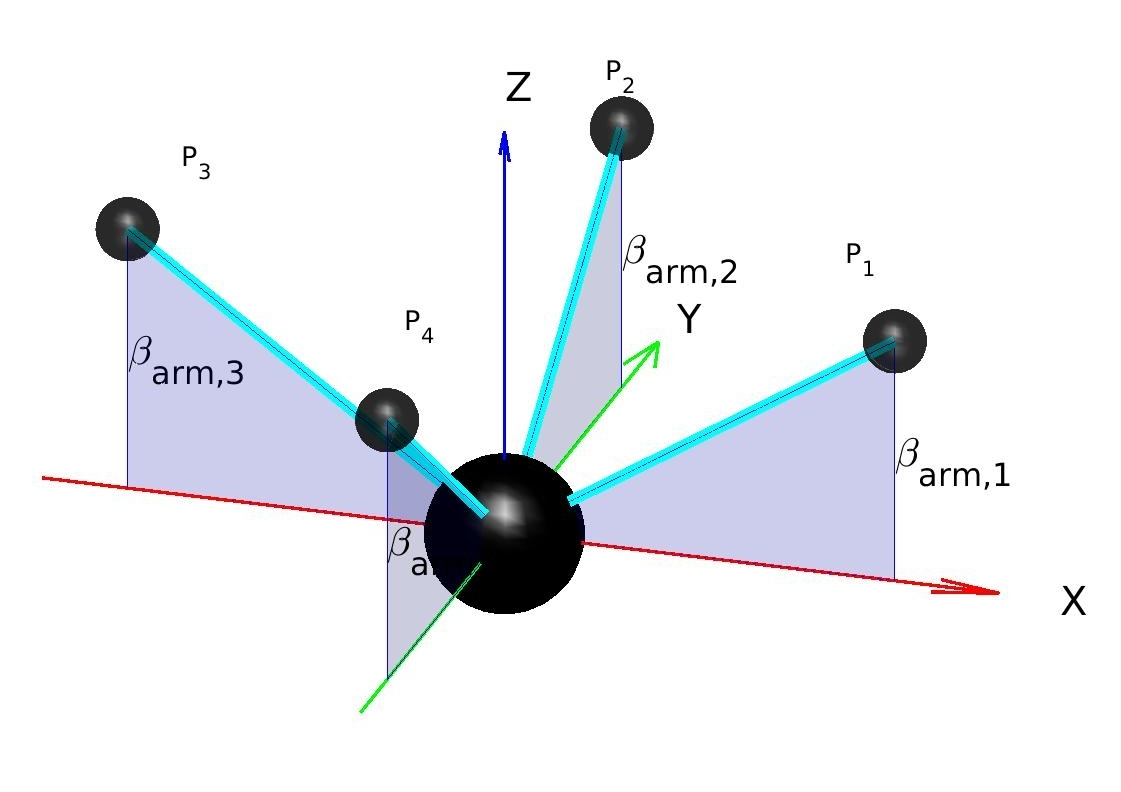
\includegraphics[width=\linewidth]{images/Quadcopter2.jpg}
    \caption{Optimal quad-copter design 2.} \label{fig:Quadcopter_resultc}
  \end{subfigure}}
  \caption{Schematic of the optimal designs obtained for the Quad-copter.}
  \label{fig:Quadcopter_result}
\end{figure}

\begin{figure}[!h]
  \resizebox{\textwidth}{!}{\begin{subfigure}[b]{0.55\textwidth}
    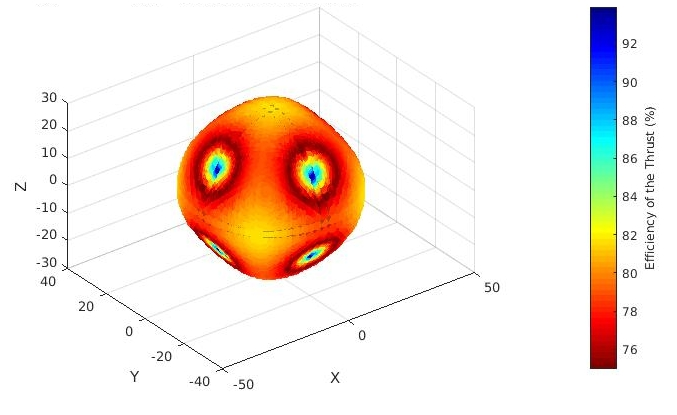
\includegraphics[width=\linewidth]{images/Quad_design_1_fspace.jpg}
    \caption{Attainable force space.} \label{fig:deisgn1_fspace}
  \end{subfigure}
  \hspace*{\fill} % separation between the subfigures
  \begin{subfigure}[b]{0.5\textwidth}
    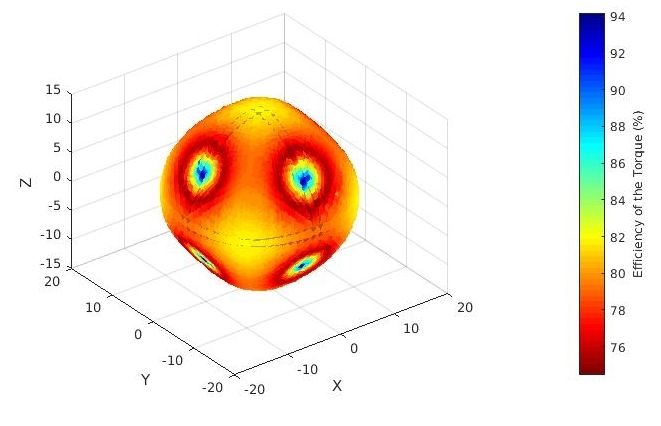
\includegraphics[width=\linewidth]{images/Quad_design_1_tspace.jpg}
    \caption{Attainable torque space.} \label{fig:deisgn1_tspace}
  \end{subfigure}
  \begin{subfigure}[b]{0.45\textwidth}
    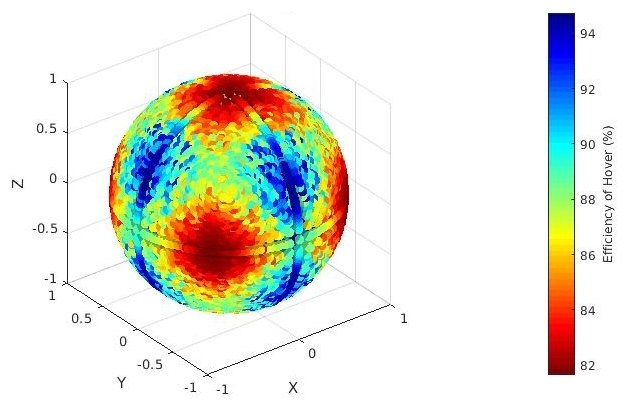
\includegraphics[width=\linewidth]{images/Quad_design_1_hspace.jpg}
    \caption{Hover efficiency in every orientation.} \label{fig:deisgn1_hspace}
  \end{subfigure}}
  \caption{Representation of the capacities of Design 1.}
  \label{fig:Quadcopter1_spaces}
\end{figure}

\begin{figure}[!h]
  \resizebox{\textwidth}{!}{\begin{subfigure}[b]{0.55\textwidth}
    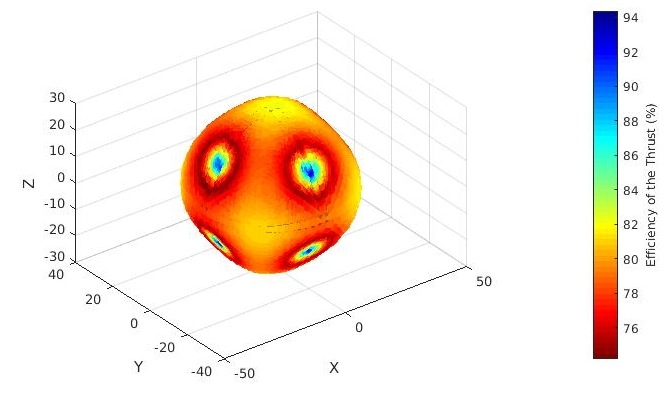
\includegraphics[width=\linewidth]{images/Quad_design_2_fspace.jpg}
    \caption{Attainable force space.} \label{fig:deisgn2_fspace}
  \end{subfigure}
  \hspace*{\fill} % separation between the subfigures
  \begin{subfigure}[b]{0.5\textwidth}
    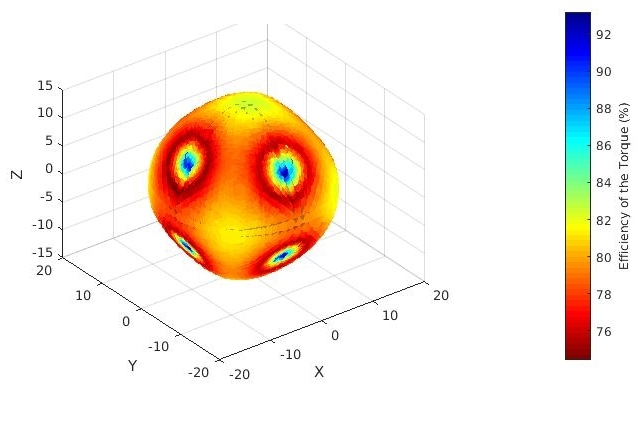
\includegraphics[width=\linewidth]{images/Quad_design_2_tspace.jpg}
    \caption{Attainable torque space.} \label{fig:deisgn2_tspace}
  \end{subfigure}
  \begin{subfigure}[b]{0.45\textwidth}
    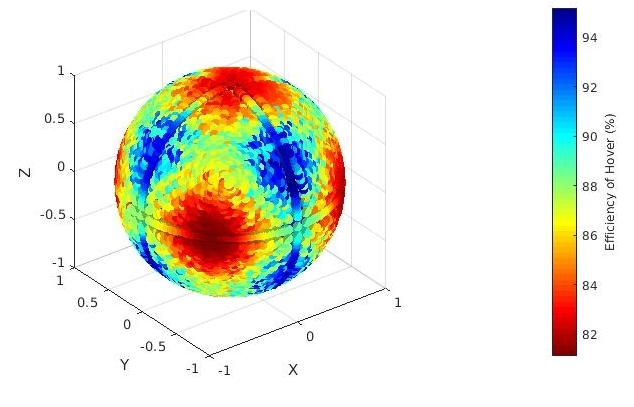
\includegraphics[width=\linewidth]{images/Quad_design_2_hspace.jpg}
    \caption{Hover efficiency in every orientation.} \label{fig:deisgn2_hspace}
  \end{subfigure}}
  \caption{Representation of the capacities of Design 2.}
  \label{fig:Quadcopter2_spaces}
\end{figure}

\begin{table}[!h]
\begin{center}
 \caption{Comparison between the two designs' force capabilities.}\vspace{1ex}
 \label{tab:tab_Quad_compare_force}
 \resizebox{\textwidth}{!}{\begin{tabular}{|l|cccccc|}
 \hline
 Design & $F_{min}\ [N]$ & $F_{max}\ [N]$ & $F_{mean}\ [N]$ & $MAD(F)\ [N]$
 & Force space volume $[N^3]$& Force space surface $[N^2]$\\ \hline
 Design 1 & 23.23 & 28.37 & 26.87 & 0.86 & 81'710 & 9'326\\
 Design 2 & 23.19 & 28.56 & 26.87 & 0.86 & 81'683 & 9'345\\
 \hline
 \end{tabular}}
\end{center}
\end{table}

\begin{table}[!h]
\begin{center}
 \caption{Comparison between the two designs' torque capabilities.}\vspace{1ex}
 \label{tab:tab_Quad_compare_torque}
 \resizebox{\textwidth}{!}{\begin{tabular}{|l|cccccc|}
 \hline
 Design & $M_{min}\ [Nm]$ & $M_{max}\ [Nm]$ & $M_{mean}\ [Nm]$ & $MAD(M)\ [Nm]$
 & Torque space volume $[N^3m^3]$ & Torque space surface $[N^2m^2]$\\ \hline
 Design 1 & 11.65 & 14.23 & 13.47 & 0.43 & 10'300 & 2'348\\
 Design 2 & 11.62 & 14.32 & 13.47 & 0.43 & 10'298 & 2'355\\
 \hline
 \end{tabular}}
\end{center}
\end{table}

\begin{table}[!h]
\begin{center}
 \caption{Comparison between the two designs' hover capabilities.}\vspace{1ex}
 \label{tab:tab_Quad_compare_hover}
 \resizebox{\textwidth}{!}{\begin{tabular}{|l|cccc|}
 \hline
  Design & $H_{eff,min}\ [\%]$ & $H_{eff,max}\ [\%]$ & $H_{eff,mean}\ [\%]$
  & $MAD(H_{eff})\ [\%]$\\ \hline
  Design 1 & 81.65 & 94.73 & 87.1 & 2.6\\
  Design 2 & 81.11 & 95.18 & 87.03 & 2.63\\
 \hline
\end{tabular}}
\end{center}
\end{table}

\subsection{Hexa-copter}
\label{sec:hexa_copter}

Optimal hexa-copter:
\begin{itemize}
  \item $n\ =\ 6$
  \item $\beta_{arm}\ =\ [35.26^{\circ},\  -35.26^{\circ},\  35.26^{\circ},\  -35.26^{\circ},\
                          35.26^{\circ},\  -35.26^{\circ}]$
  \item $\theta_{arm}\ =\ [0^{\circ},\  0^{\circ},\  0^{\circ},\  0^{\circ},\ 0^{\circ},\  0^{\circ}]$
  \item $L\ =\ 0.5\ [m]$
\end{itemize}

Voliro:
\begin{itemize}
  \item $n\ =\ 6$
  \item $\beta_{arm}\ =\ [0^{\circ},\  0^{\circ},\  0^{\circ},\  0^{\circ},\ 0^{\circ},\  0^{\circ}]$
  \item $\theta_{arm}\ =\ [0^{\circ},\  0^{\circ},\  0^{\circ},\  0^{\circ},\ 0^{\circ},\  0^{\circ}]$
  \item $L\ =\ 0.5\ [m]$
\end{itemize}

\begin{figure}[!h]
  \resizebox{\textwidth}{!}{\begin{subfigure}[b]{0.55\textwidth}
    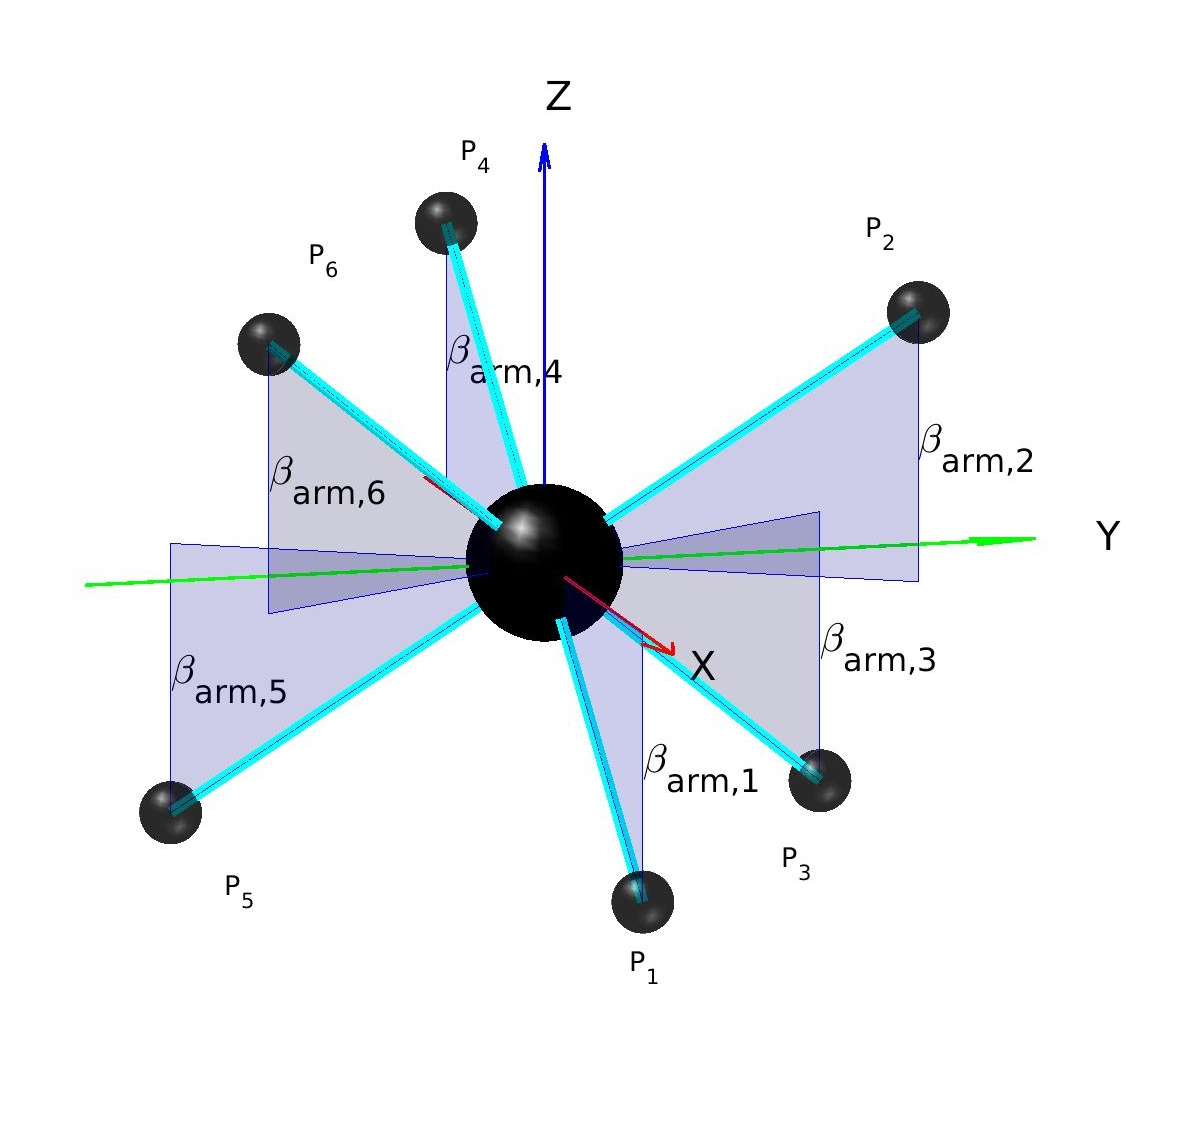
\includegraphics[width=\linewidth]{images/Hexacopter.jpg}
    \caption{Optimal hexa-copter} \label{fig:Hexacopter_resulta}
  \end{subfigure}
  \hspace*{\fill} % separation between the subfigures
  \begin{subfigure}[b]{0.5\textwidth}
    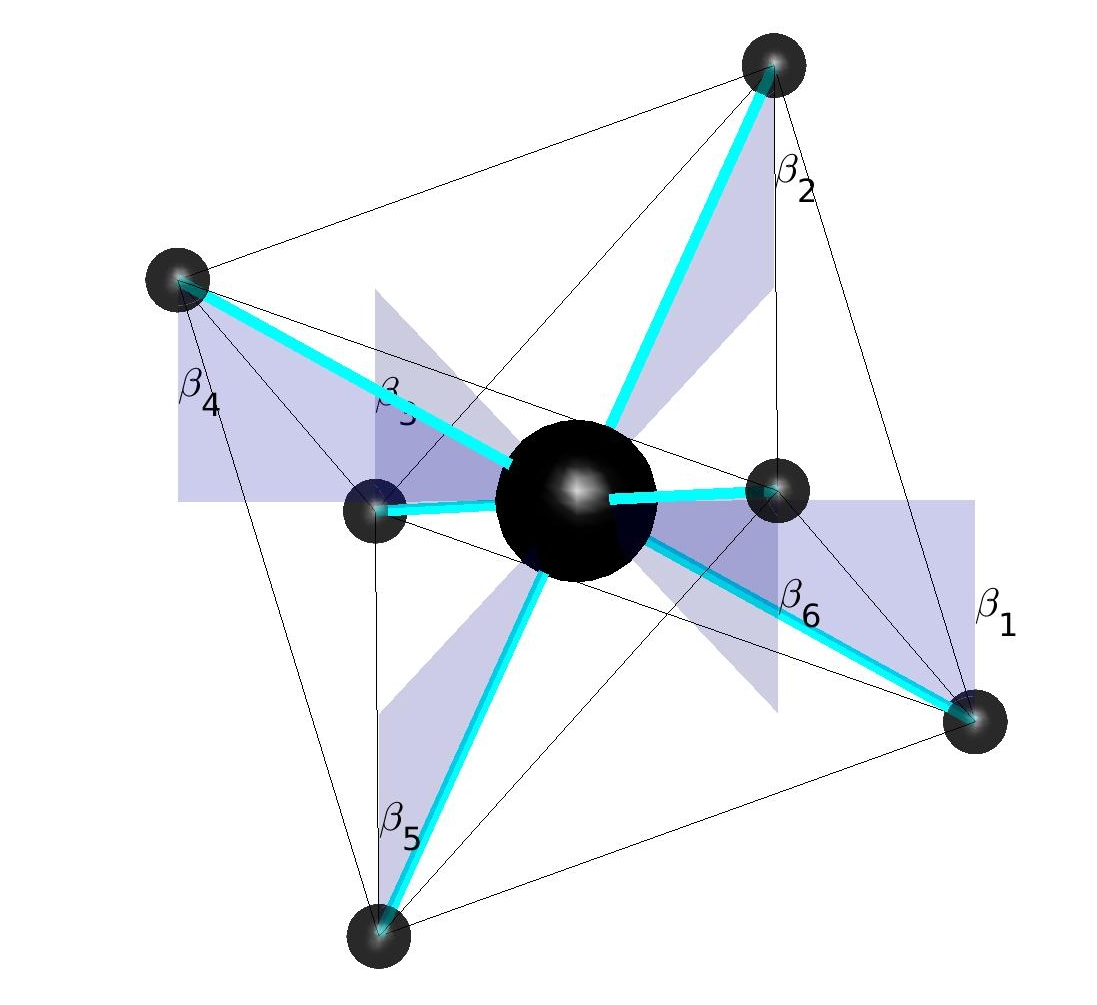
\includegraphics[width=\linewidth]{images/Hexa_octahedron.jpg}
    \caption{Hexa-copter in an octahedron.} \label{fig:Hexacopter_resultb}
  \end{subfigure}
  \hspace*{\fill} % separation between the subfigures
  \begin{subfigure}[b]{0.7\textwidth}
    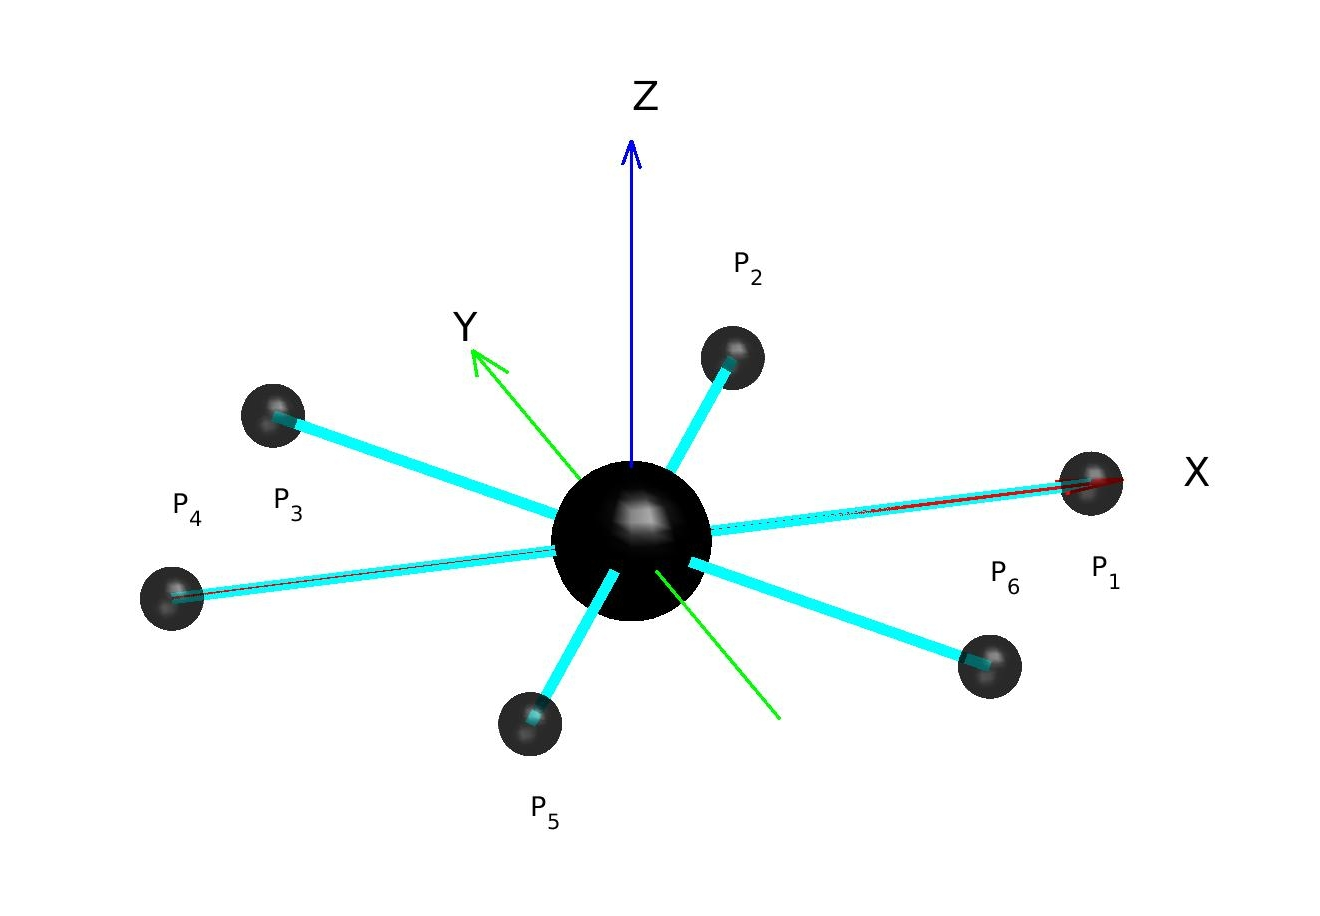
\includegraphics[width=\linewidth]{images/Voliro.jpg}
    \caption{Voliro's design for comparison.} \label{fig:Hexacopter_resultc}
  \end{subfigure}}
  \caption{Schematic of the differnt possible designs for an Hexa-copter.}
  \label{fig:Hexacopter_result}
\end{figure}

\begin{figure}[!h]
  \resizebox{\textwidth}{!}{\begin{subfigure}[b]{0.55\textwidth}
    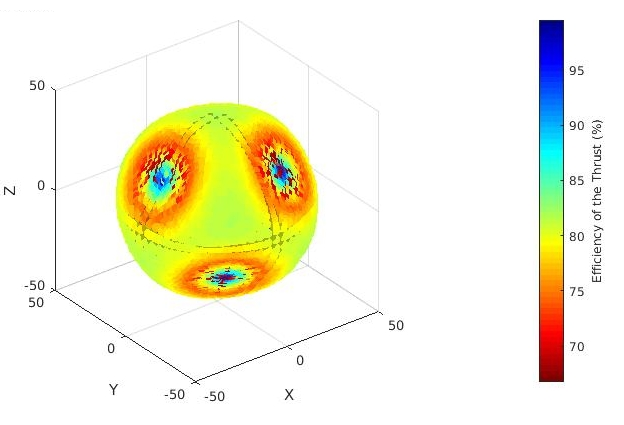
\includegraphics[width=\linewidth]{images/Hexa_fspace.jpg}
    \caption{Attainable force space.} \label{fig:hexa_fspace}
  \end{subfigure}
  \hspace*{\fill} % separation between the subfigures
  \begin{subfigure}[b]{0.5\textwidth}
    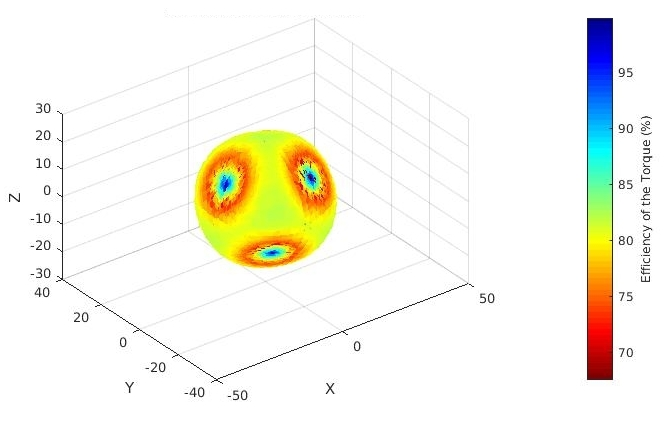
\includegraphics[width=\linewidth]{images/Hexa_tspace.jpg}
    \caption{Attainable torque space.} \label{fig:hexa_tspace}
  \end{subfigure}
  \begin{subfigure}[b]{0.45\textwidth}
    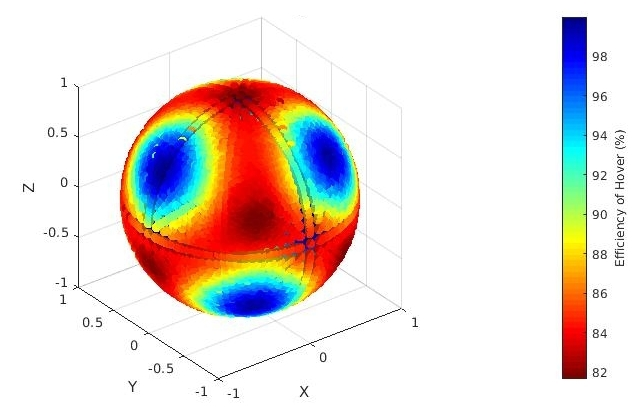
\includegraphics[width=\linewidth]{images/Hexa_hspace.jpg}
    \caption{Hover efficiency in every orientation.} \label{fig:hexa_hspace}
  \end{subfigure}}
  \caption{Representation of the capacities of the optimal hexa-copter.}
  \label{fig:Hexacopter_spaces}
\end{figure}

\begin{figure}[!h]
  \resizebox{\textwidth}{!}{\begin{subfigure}[b]{0.55\textwidth}
    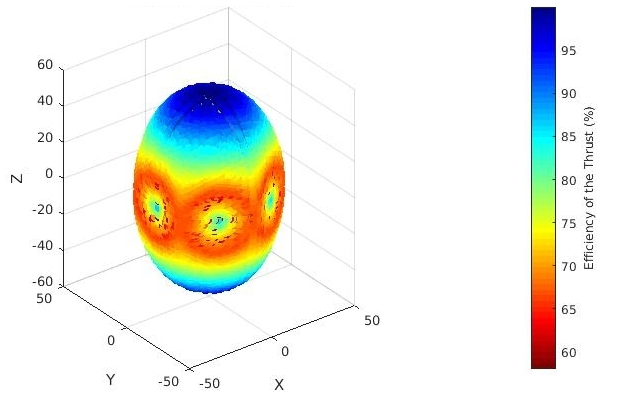
\includegraphics[width=\linewidth]{images/Voliro_fspace.jpg}
    \caption{Attainable force space.} \label{fig:voliro_fspace}
  \end{subfigure}
  \hspace*{\fill} % separation between the subfigures
  \begin{subfigure}[b]{0.5\textwidth}
    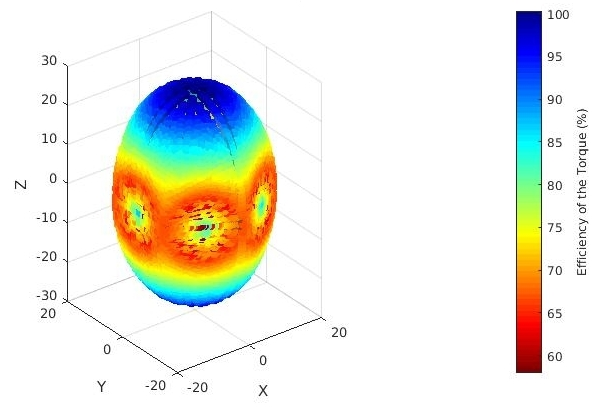
\includegraphics[width=\linewidth]{images/Voliro_tspace.jpg}
    \caption{Attainable torque space.} \label{fig:voliro_tspace}
  \end{subfigure}
  \begin{subfigure}[b]{0.45\textwidth}
    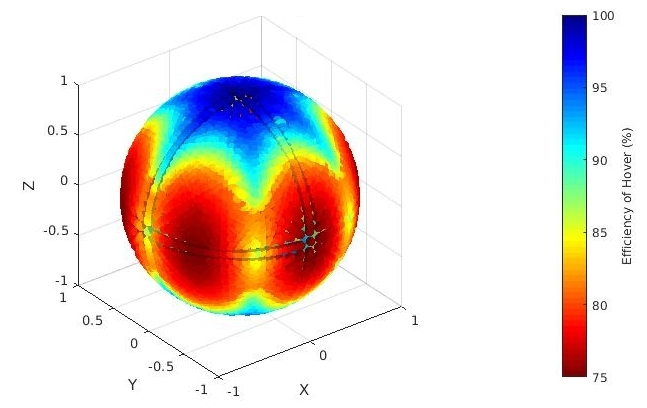
\includegraphics[width=\linewidth]{images/Voliro_hspace.jpg}
    \caption{Hover efficiency in every orientation.} \label{fig:voliro_hspace}
  \end{subfigure}}
  \caption{Representation of the capacities of Voliro.}
  \label{fig:Voliro_spaces}
\end{figure}

\begin{table}[!h]
\begin{center}
 \caption{Comparison between the two designs' force capabilities.}\vspace{1ex}
 \label{tab:tab_Hexa_compare_force}
 \resizebox{\textwidth}{!}{\begin{tabular}{|l|cccccc|}
 \hline
 Design & $F_{min}\ [N]$ & $F_{max}\ [N]$ & $F_{mean}\ [N]$ & $MAD(F)\ [N]$
 & Force space volume $[N^3]$& Force space surface $[N^2]$\\ \hline
 Optimal hexa-copter & 34.74 & 42.55 & 39.52 & 2.21 & 267'010 & 20'922\\
 Voliro & 26.6 & 52.11 & 37.77 & 4.33 & 244'293 & 20'170\\
 \hline
 \end{tabular}}
\end{center}
\end{table}

\begin{table}[!h]
\begin{center}
 \caption{Comparison between the two designs' torque capabilities.}\vspace{1ex}
 \label{tab:tab_Hexa_compare_torque}
 \resizebox{\textwidth}{!}{\begin{tabular}{|l|cccccc|}
 \hline
 Design & $M_{min}\ [Nm]$ & $M_{max}\ [Nm]$ & $M_{mean}\ [Nm]$ & $MAD(M)\ [Nm]$
 & Torque space volume $[N^3m^3]$ & Torque space surface $[N^2m^2]$\\ \hline
 Optimal hexa-copter & 17.42 & 21.34 & 19.82 & 1.1 & 33'687 & 5'230\\
 Voliro & 15.09 & 26.13 & 18.94 & 2.17 & 30'788 & 5'121\\
 \hline
 \end{tabular}}
\end{center}
\end{table}

\begin{table}[!h]
\begin{center}
 \caption{Comparison between two designs' hover capabilities.}\vspace{1ex}
 \label{tab:tab_Hexa_compare_hover}
 \resizebox{\textwidth}{!}{\begin{tabular}{|l|cccc|}
 \hline
  Design & $H_{eff,min}\ [\%]$ & $H_{eff,max}\ [\%]$ & $H_{eff,mean}\ [\%]$
  & $MAD(H_{eff})\ [\%]$\\ \hline
  Optimal hexa-copter & 81.65 & 100 & 88.92 & 4.43\\
  Voliro & 75 & 100 & 84.21 & 5.35\\
 \hline
\end{tabular}}
\end{center}
\end{table}

\subsection{Octa-copter}
\label{sec:octa_copter}

Optimal octa-copter:
\begin{itemize}
  \item $n\ =\ 8$
  \item $\beta_{arm}\ =\ [35.26^{\circ},\  -35.26^{\circ},\  35.26^{\circ},\  -35.26^{\circ},\
                          35.26^{\circ},\  -35.26^{\circ},\ 35.26^{\circ},\  -35.26^{\circ}]$
  \item $\theta_{arm}\ =\ [0^{\circ},\  0^{\circ},\  0^{\circ},\  0^{\circ},\ 0^{\circ},\  0^{\circ},\ 0^{\circ},\  0^{\circ}]$
  \item $L\ =\ 0.5\ [m]$
\end{itemize}

Omnicopter:
\begin{itemize}
  \item $n\ =\ 8$
  \item $\beta_{arm}\ =\ [-35.26^{\circ},\  -35.26^{\circ},\  -35.26^{\circ},\  -35.26^{\circ},\
                          35.26^{\circ},\  35.26^{\circ},\ 35.26^{\circ},\  35.26^{\circ}]$
  \item $\theta_{arm}\ =\ [0^{\circ},\  45^{\circ},\  90^{\circ},\  135^{\circ},\
                          180^{\circ},\  -135^{\circ},\ -90^{\circ},\  -45^{\circ}]$
  \item $L\ =\ 0.5\ [m]$
\end{itemize}

\begin{figure}[!h]
  \resizebox{\textwidth}{!}{\begin{subfigure}[b]{0.6\textwidth}
    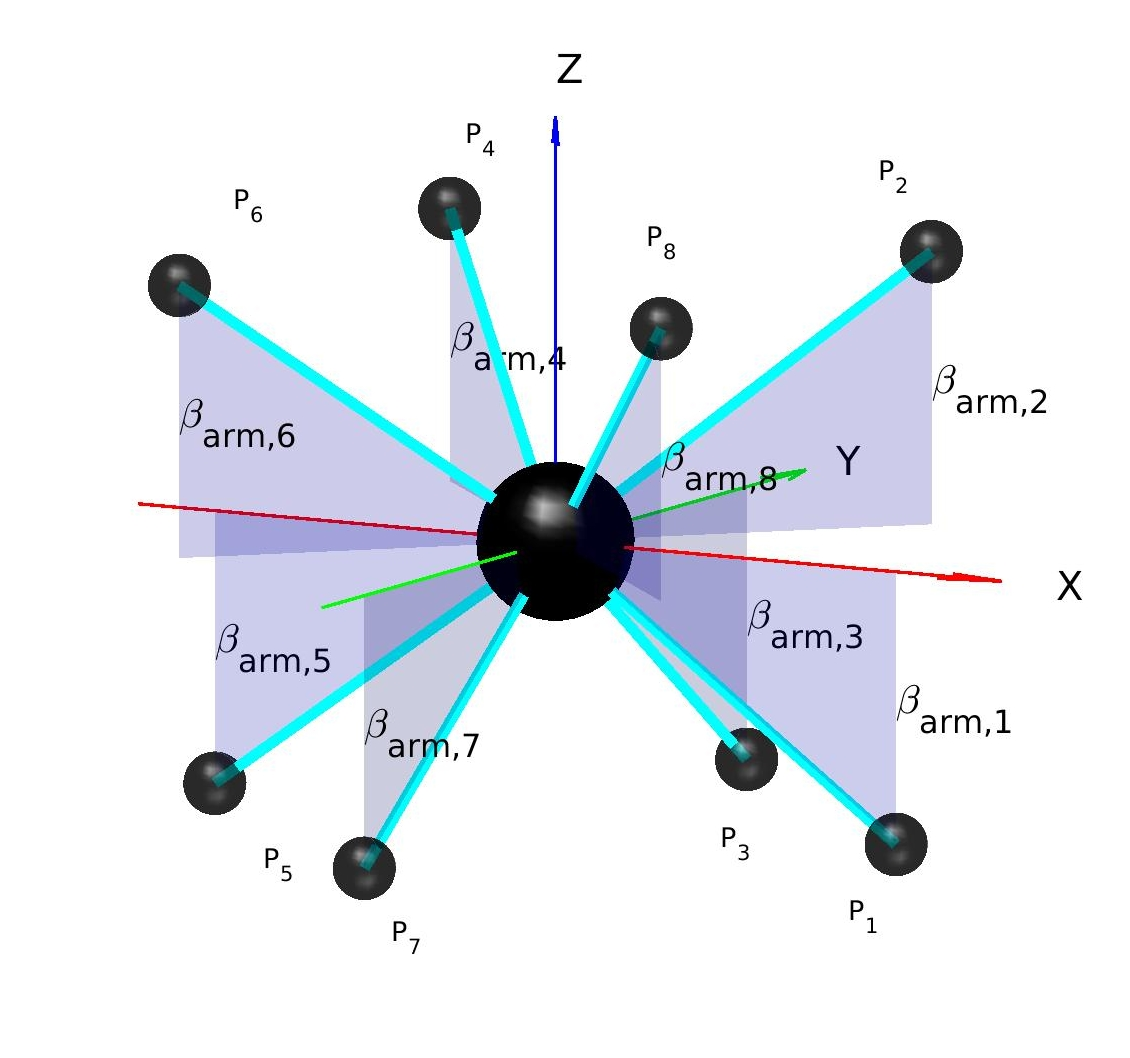
\includegraphics[width=\linewidth]{images/Octacopter.jpg}
    \caption{Optimal hexa-copter} \label{fig:Octacopter_resulta}
  \end{subfigure}
  \hspace*{\fill} % separation between the subfigures
  \begin{subfigure}[b]{0.6\textwidth}
    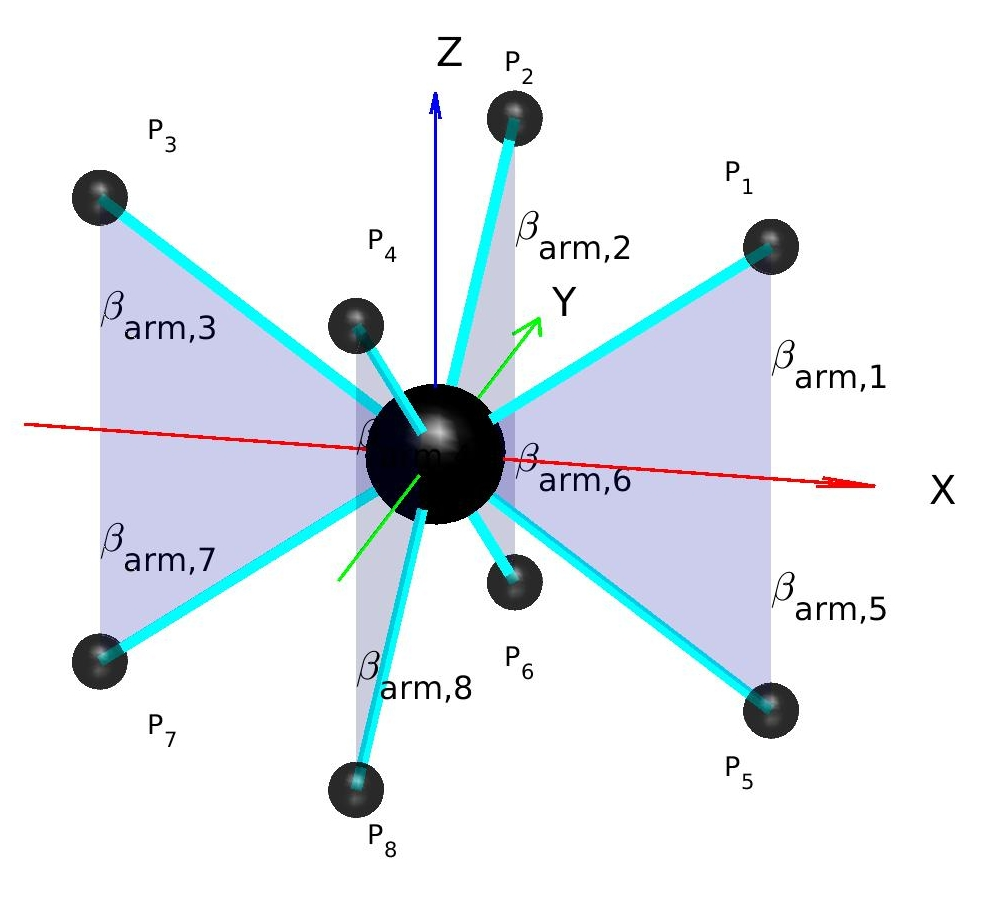
\includegraphics[width=\linewidth]{images/omnicopter.jpg}
    \caption{Omnicopter's design for comparison.} \label{fig:Octacopter_resultb}
  \end{subfigure}
  \hspace*{\fill} % separation between the subfigures
  \begin{subfigure}[b]{0.5\textwidth}
    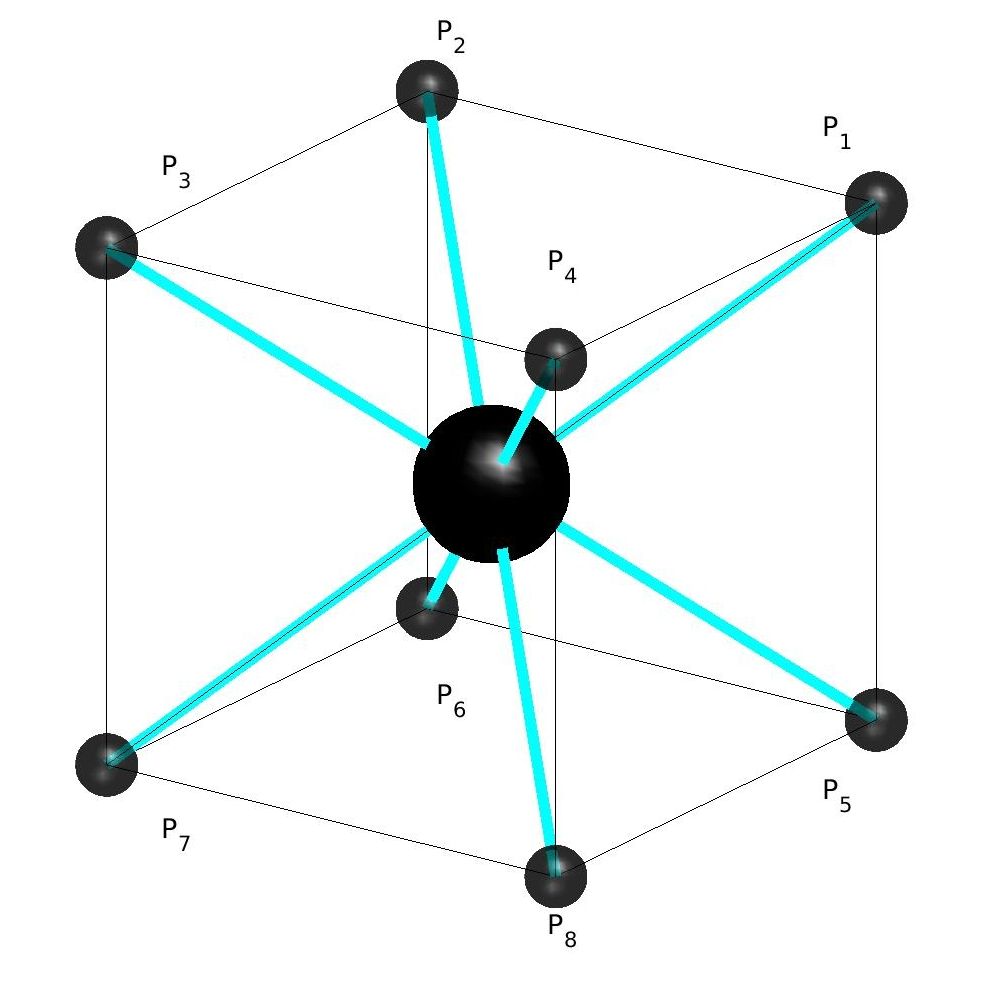
\includegraphics[width=\linewidth]{images/Octa_cube.jpg}
    \caption{Omnicopter in a cube.} \label{fig:Octacopter_resultc}
  \end{subfigure}}
  \caption{Schematic of the differnt possible designs for an Octa-copter.}
  \label{fig:Octacopter_result}
\end{figure}

\begin{figure}[!h]
  \resizebox{\textwidth}{!}{\begin{subfigure}[b]{0.55\textwidth}
    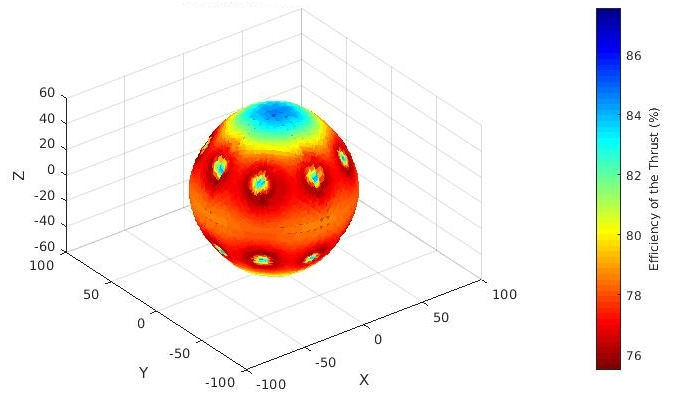
\includegraphics[width=\linewidth]{images/Octa_fspace.jpg}
    \caption{Attainable force space.} \label{fig:Octa_fspace}
  \end{subfigure}
  \hspace*{\fill} % separation between the subfigures
  \begin{subfigure}[b]{0.5\textwidth}
    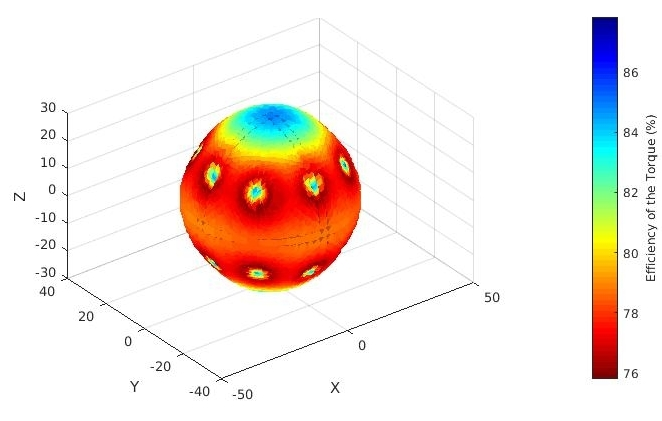
\includegraphics[width=\linewidth]{images/Octa_tspace.jpg}
    \caption{Attainable torque space.} \label{fig:Octa_tspace}
  \end{subfigure}
  \begin{subfigure}[b]{0.45\textwidth}
    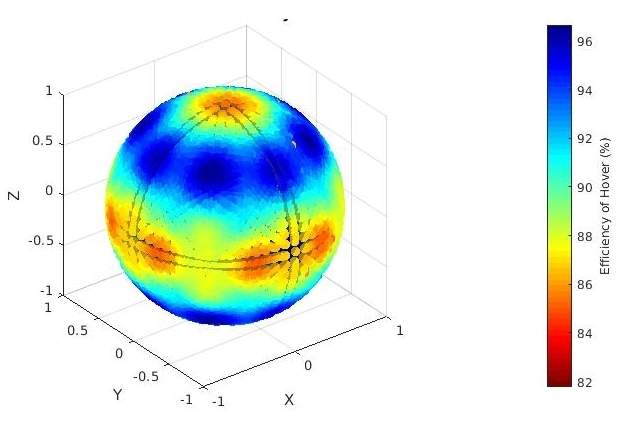
\includegraphics[width=\linewidth]{images/Octa_hspace.jpg}
    \caption{Hover efficiency in every orientation.} \label{fig:Octa_hspace}
  \end{subfigure}}
  \caption{Representation of the capacities of the optimal octa-copter.}
  \label{fig:Octacopter_spaces}
\end{figure}

\begin{figure}[!h]
  \resizebox{\textwidth}{!}{\begin{subfigure}[b]{0.55\textwidth}
    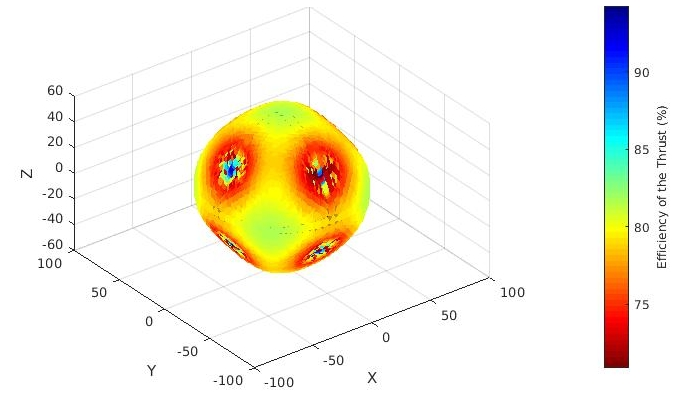
\includegraphics[width=\linewidth]{images/Omnicopter_fspace.jpg}
    \caption{Attainable force space.} \label{fig:Omnicopter_fspace}
  \end{subfigure}
  \hspace*{\fill} % separation between the subfigures
  \begin{subfigure}[b]{0.5\textwidth}
    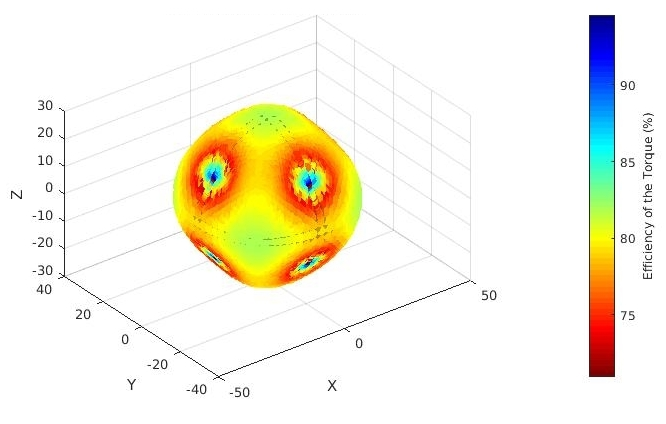
\includegraphics[width=\linewidth]{images/Omnicopter_tspace.jpg}
    \caption{Attainable torque space.} \label{fig:Omnicopter_tspace}
  \end{subfigure}
  \begin{subfigure}[b]{0.45\textwidth}
    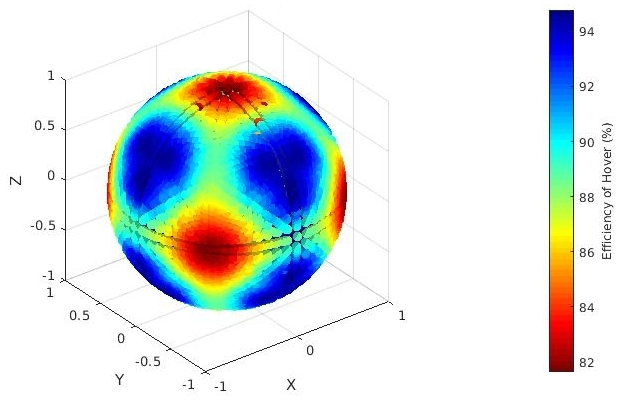
\includegraphics[width=\linewidth]{images/Omnicopter_hspace.jpg}
    \caption{Hover efficiency in every orientation.} \label{fig:Omnicopter_hspace}
  \end{subfigure}}
  \caption{Representation of the capacities of Omnicopter.}
  \label{fig:Omnicopter_spaces}
\end{figure}

\begin{table}[!h]
\begin{center}
 \caption{Comparison between the two designs' force capabilities.}\vspace{1ex}
 \label{tab:tab_Octa_compare_force}
 \resizebox{\textwidth}{!}{\begin{tabular}{|l|cccccc|}
 \hline
 Design & $F_{min}\ [N]$ & $F_{max}\ [N]$ & $F_{mean}\ [N]$ & $MAD(F)\ [N]$
 & Force space volume $[N^3]$& Force space surface $[N^2]$\\ \hline
 Optimal octa-copter & 44.7 & 58.78 & 53.95 & 0.94 & 669'339 & 37'625\\
 Omnicopter & 46.46 & 56.73 & 53.75 & 1.72 & 653'736 & 37'263\\
 \hline
 \end{tabular}}
\end{center}
\end{table}

\begin{table}[!h]
\begin{center}
 \caption{Comparison between the two designs' torque capabilities.}\vspace{1ex}
 \label{tab:tab_Octa_compare_torque}
 \resizebox{\textwidth}{!}{\begin{tabular}{|l|cccccc|}
 \hline
 Design & $M_{min}\ [Nm]$ & $M_{max}\ [Nm]$ & $M_{mean}\ [Nm]$ & $MAD(M)\ [Nm]$
 & Torque space volume $[N^3m^3]$ & Torque space surface $[N^2m^2]$\\ \hline
 Optimal octa-copter & 22.4 & 29.48 & 27 & 0.47 & 84'417 & 9'463\\
 Omnicopter & 23.3 & 28.45 & 26.95 & 0.86 & 82'446 & 9'374\\
 \hline
 \end{tabular}}
\end{center}
\end{table}

\begin{table}[!h]
\begin{center}
 \caption{Comparison between two designs' hover capabilities.}\vspace{1ex}
 \label{tab:tab_Octa_compare_hover}
 \resizebox{\textwidth}{!}{\begin{tabular}{|l|cccc|}
 \hline
  Design & $H_{eff,min}\ [\%]$ & $H_{eff,max}\ [\%]$ & $H_{eff,mean}\ [\%]$
  & $MAD(H_{eff})\ [\%]$\\ \hline
  Optimal octa-copter & 81.78 & 96.65 & 91.42 & 2.7\\
  Omnicopter & 81.64 & 94.77 & 89.36 & 2.82\\
 \hline
\end{tabular}}
\end{center}
\end{table}

\section{Odd Designs}
\label{sec:odd_designs}

\subsection{Tri-copter}
\label{sec:tri_copter}
Optimal tri-copter:
\begin{itemize}
  \item $n\ =\ 3$
  \item $\beta_{arm}\ =\ [35.26^{\circ},\  35.26^{\circ},\  35.26^{\circ}]$
  \item $\theta_{arm}\ =\ [0^{\circ},\  0^{\circ},\  0^{\circ}]$
  \item $L\ =\ 0.5\ [m]$
\end{itemize}

\begin{figure}[!h]
  \resizebox{\textwidth}{!}{\begin{subfigure}[b]{0.45\textwidth}
    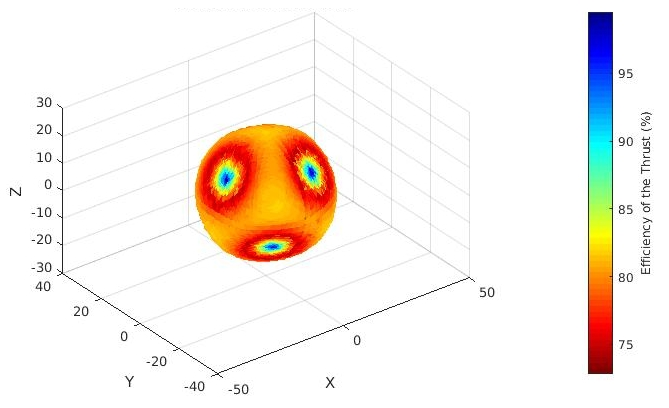
\includegraphics[width=\linewidth]{images/Tri_fspace.jpg}
    \caption{Force space.} \label{fig:Tricopter_fspace}
  \end{subfigure}
  \hspace*{\fill} % separation between the subfigures
  \begin{subfigure}[b]{0.4\textwidth}
    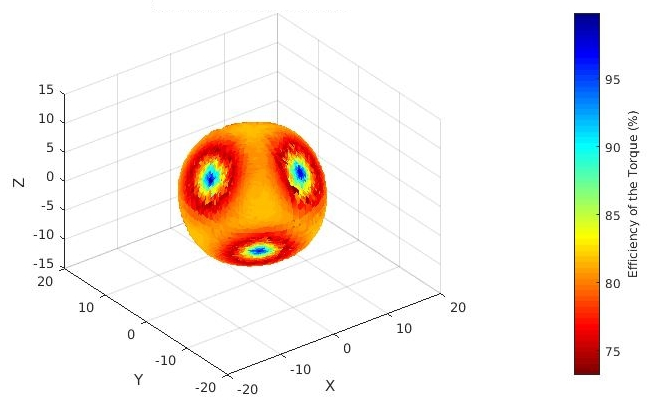
\includegraphics[width=\linewidth]{images/Tri_tspace.jpg}
    \caption{Torque space.} \label{fig:Tricopter_tspace}
  \end{subfigure}}
  \hspace*{\fill} % separation between the subfigures
  \resizebox{\textwidth}{!}{\begin{subfigure}[b]{0.4\textwidth}
    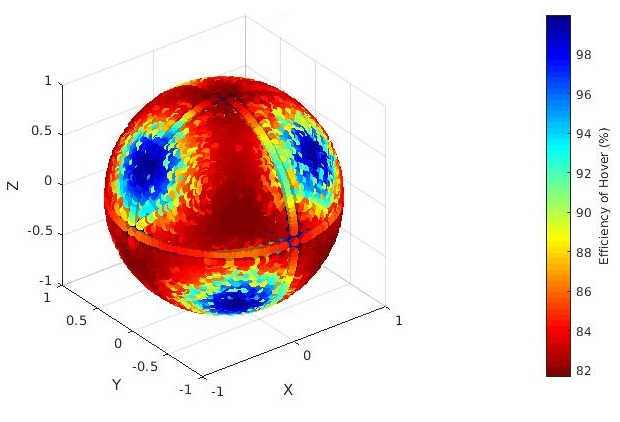
\includegraphics[width=\linewidth]{images/Tri_hspace.jpg}
    \caption{Hover efficiency space.} \label{fig:Tricopter_hspace}
  \end{subfigure}
  \hspace*{\fill} % separation between the subfigures
  \begin{subfigure}[b]{0.4\textwidth}
    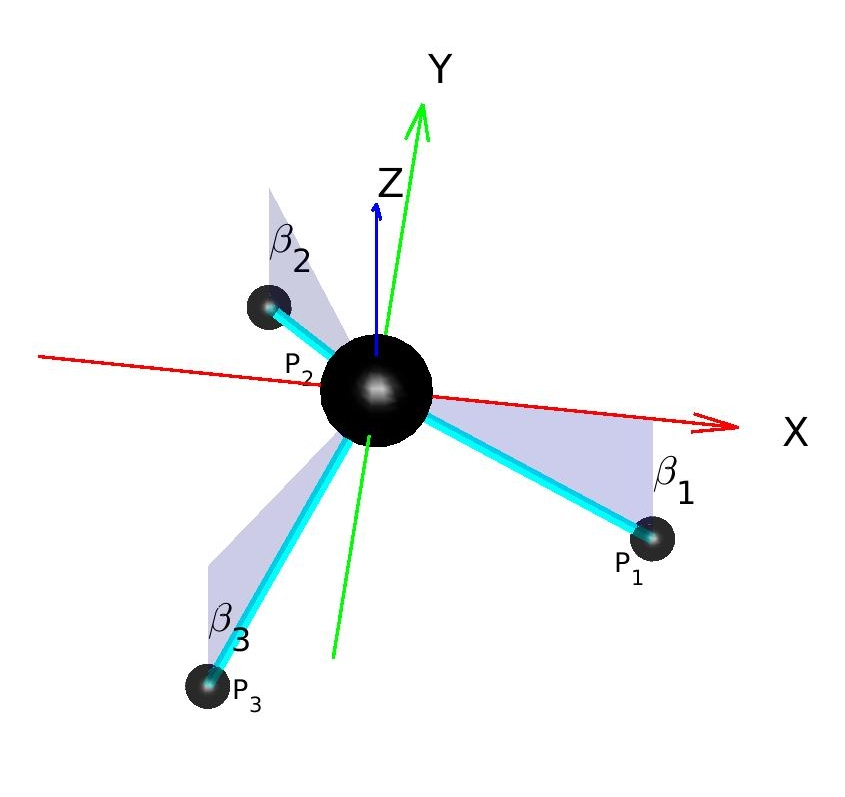
\includegraphics[width=\linewidth]{images/Tricopter.jpg}
    \caption{Design representation.} \label{fig:Tricopter_visual}
  \end{subfigure}}
  \caption{Visual representation of the optimal tri-copter capabilities.}
  \label{fig:Tricopter_result}
\end{figure}

\begin{table}[!h]
 \caption{Information on the optimal tri-copter.}\vspace{1ex}
 \label{tab:tab_Tri_metrics}
 \begin{center}
 \resizebox{\textwidth}{!}{\begin{tabular}{|cccccc|}
 \hline
 $F_{min}\ [N]$ & $F_{max}\ [N]$ & $F_{mean}\ [N]$ & $MAD(F)\ [N]$
 & Force space volume $[N^3]$& Force space surface $[N^2]$\\ \hline
 17.37 & 21.27 & 19.73 & 1.1 & 33'217 & 5'313\\
 \hline
 \end{tabular}}
 \resizebox{\textwidth}{!}{\begin{tabular}{|cccccc|}
 \hline
 $M_{min}\ [Nm]$ & $M_{max}\ [Nm]$ & $M_{mean}\ [Nm]$ & $MAD(M)\ [Nm]$
 & Torque space volume $[N^3m^3]$ & Torque space surface $[N^2m^2]$\\ \hline
 8.7 & 10.67 & 9.87 & 0.56 & 4'158 & 1'379\\
 \hline
 \end{tabular}}
 {\tiny\begin{tabular}{|cccc|}
 \hline
  $H_{eff,min}\ [\%]$ & $H_{eff,max}\ [\%]$ & $H_{eff,mean}\ [\%]$
  & $MAD(H_{eff})\ [\%]$\\ \hline
  81.65 & 99 & 87.22 & 4.42\\
 \hline
\end{tabular}}
\end{center}
\end{table}

\subsection{Penta-copter}
\label{sec:penta_copter}
Optimal penta-copter:
\begin{itemize}
  \item $n\ =\ 5$
  \item $\beta_{arm}\ =\ [35.26^{\circ},\  35.26^{\circ},\  35.26^{\circ},\  35.26^{\circ},\   35.26^{\circ}]$
  \item $\theta_{arm}\ =\ [0^{\circ},\  0^{\circ},\  0^{\circ},\  0^{\circ},\  0^{\circ}]$
  \item $L\ =\ 0.5\ [m]$
\end{itemize}

Standard penta-copter:
\begin{itemize}
  \item $n\ =\ 5$
  \item $\beta_{arm}\ =\ [0^{\circ},\  0^{\circ},\  0^{\circ},\  0^{\circ},\  0^{\circ}]$
  \item $\theta_{arm}\ =\ [0^{\circ},\  0^{\circ},\  0^{\circ},\  0^{\circ},\  0^{\circ}]$
  \item $L\ =\ 0.5\ [m]$
\end{itemize}
\begin{figure}[!h]
  \begin{subfigure}[b]{0.4\textwidth}
    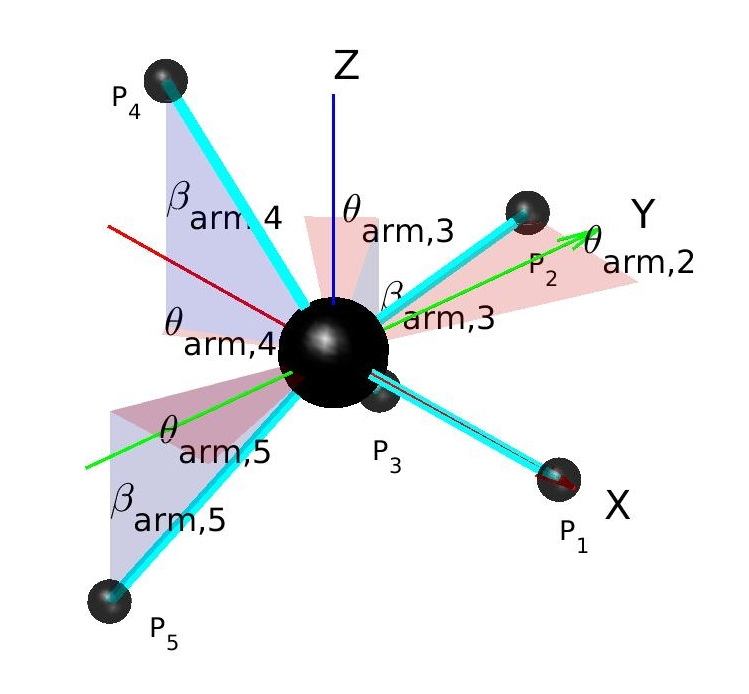
\includegraphics[width=\linewidth]{images/Pentacopter_odd.jpg}
    \caption{Optimal hexa-copter.} \label{fig:Pentacopter_odd}
  \end{subfigure}
  \hspace*{\fill} % separation between the subfigures
  \begin{subfigure}[b]{0.5\textwidth}
    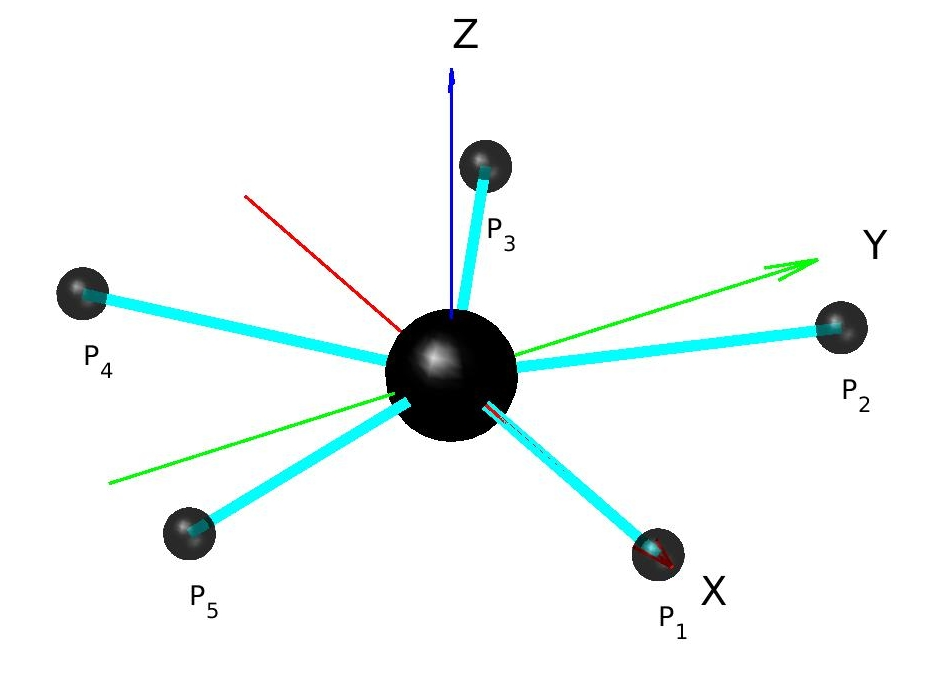
\includegraphics[width=\linewidth]{images/Pentacopter_standard.jpg}
    \caption{Hexa-copter standard.} \label{fig:Pentacopter_standard}
  \end{subfigure}
  \caption{Schematic of different possible designs for a Penta-copter.}
  \label{fig:Pentacopter_result}
\end{figure}

\begin{table}[!h]
\begin{center}
 \caption{Comparison between the two designs' force capabilities.}\vspace{1ex}
 \label{tab:tab_Penta_compare_force}
 \resizebox{\textwidth}{!}{\begin{tabular}{|l|cccccc|}
 \hline
 Design & $F_{min}\ [N]$ & $F_{max}\ [N]$ & $F_{mean}\ [N]$ & $MAD(F)\ [N]$
 & Force space volume $[N^3]$& Force space surface $[N^2]$\\ \hline
 Design 1 & 26.03 & 36.22 & 33.69 & 1.39 & 160'333 & 14'626\\
 Standard & 26.24 & 43.42 & 31.93 & 3.25 & 146'006 & 14'137\\
 \hline
 \end{tabular}}
\end{center}
\end{table}

\begin{table}[!h]
\begin{center}
 \caption{Comparison between the two designs' torque capabilities.}\vspace{1ex}
 \label{tab:tab_Penta_compare_torque}
 \resizebox{\textwidth}{!}{\begin{tabular}{|l|cccccc|}
 \hline
 Design & $M_{min}\ [Nm]$ & $M_{max}\ [Nm]$ & $M_{mean}\ [Nm]$ & $MAD(M)\ [Nm]$
 & Torque space volume $[N^3m^3]$ & Torque space surface $[N^2m^2]$\\ \hline
 Optimal & 12.85 & 18.2 & 16.93 & 0.7 & 20'358 & 3'741\\
 Standard & 10.9 & 21.8 & 16 & 1.63 & 18'409 & 3'580\\
 \hline
 \end{tabular}}
\end{center}
\end{table}

\begin{table}[!h]
\begin{center}
 \caption{Comparison between two designs' hover capabilities.}\vspace{1ex}
 \label{tab:tab_Penta_compare_hover}
 \resizebox{\textwidth}{!}{\begin{tabular}{|l|cccc|}
 \hline
  Design & $H_{eff,min}\ [\%]$ & $H_{eff,max}\ [\%]$ & $H_{eff,mean}\ [\%]$
  & $MAD(H_{eff})\ [\%]$\\ \hline
  Optimal & 80.33 & 99.4 & 90.96 & 3\\
  Standard & 77.25 & 100 & 84.38 & 5.2\\
 \hline
\end{tabular}}
\end{center}
\end{table}

\subsection{Hepta-copter}
\label{sec:hepta_copter}
\begin{table}[!h]
\begin{center}
 \caption{Comparison between the two designs' force capabilities.}\vspace{1ex}
 \label{tab:tab_hepta_compare_force}
 \resizebox{\textwidth}{!}{\begin{tabular}{|l|cccccc|}
 \hline
 Design & $F_{min}\ [N]$ & $F_{max}\ [N]$ & $F_{mean}\ [N]$ & $MAD(F)\ [N]$
 & Force space volume $[N^3]$& Force space surface $[N^2]$\\ \hline
 Optimal hepta-copter &  &  &  &  &  & \\
 Standard hepta-copter &  &  &  &  &  & \\
 \hline
 \end{tabular}}
\end{center}
\end{table}

\begin{table}[!h]
\begin{center}
 \caption{Comparison between the two designs' torque capabilities.}\vspace{1ex}
 \label{tab:tab_hepta_compare_torque}
 \resizebox{\textwidth}{!}{\begin{tabular}{|l|cccccc|}
 \hline
 Design & $M_{min}\ [Nm]$ & $M_{max}\ [Nm]$ & $M_{mean}\ [Nm]$ & $MAD(M)\ [Nm]$
 & Torque space volume $[N^3m^3]$ & Torque space surface $[N^2m^2]$\\ \hline
 Optimal hepta-copter &  &  &  &  &  & \\
 Standard hepta-copter &  &  &  &  &  & \\
 \hline
 \end{tabular}}
\end{center}
\end{table}

\begin{table}[!h]
\begin{center}
 \caption{Comparison between two designs' hover capabilities.}\vspace{1ex}
 \label{tab:tab_hepta_compare_hover}
 \resizebox{\textwidth}{!}{\begin{tabular}{|l|cccc|}
 \hline
  Design & $H_{eff,min}\ [\%]$ & $H_{eff,max}\ [\%]$ & $H_{eff,mean}\ [\%]$
  & $MAD(H_{eff})\ [\%]$\\ \hline
  Optimal hepta-copter &  &  &  &  \\
  Standard hepta-copter &  &  &  &  \\
 \hline
\end{tabular}}
\end{center}
\end{table}

\section{Comparison of Different Designs}
\label{sec:comparison}
\begin{table}[!h]
\begin{center}
 \caption{Comparison between the two designs' force capabilities.}\vspace{1ex}
 \label{tab:tab_all_compare_force}
 \resizebox{\textwidth}{!}{\begin{tabular}{|l|cccccc|}
 \hline
 Design & $F_{min}\ [N]$ & $F_{max}\ [N]$ & $F_{mean}\ [N]$ & $MAD(F)\ [N]$
 & Force space volume $[N^3]$& Force space surface $[N^2]$\\ \hline
 Optimal octa-copter &  &  &  &  &  & \\
 Omnicopter &  &  &  &  &  & \\
 \hline
 \end{tabular}}
\end{center}
\end{table}

\begin{table}[!h]
\begin{center}
 \caption{Comparison between the two designs' torque capabilities.}\vspace{1ex}
 \label{tab:tab_all_compare_torque}
 \resizebox{\textwidth}{!}{\begin{tabular}{|l|cccccc|}
 \hline
 Design & $M_{min}\ [Nm]$ & $M_{max}\ [Nm]$ & $M_{mean}\ [Nm]$ & $MAD(M)\ [Nm]$
 & Torque space volume $[N^3m^3]$ & Torque space surface $[N^2m^2]$\\ \hline
 Optimal octa-copter &  &  &  &  &  & \\
 Omnicopter &  &  &  &  &  & \\
 \hline
 \end{tabular}}
\end{center}
\end{table}

\begin{table}[!h]
\begin{center}
 \caption{Comparison between two designs' hover capabilities.}\vspace{1ex}
 \label{tab:tab_all_compare_hover}
 \resizebox{\textwidth}{!}{\begin{tabular}{|l|cccc|}
 \hline
  Design & $H_{eff,min}\ [\%]$ & $H_{eff,max}\ [\%]$ & $H_{eff,mean}\ [\%]$
  & $MAD(H_{eff})\ [\%]$\\ \hline
  Optimal octa-copter &  &  &  &  \\
  Omnicopter &  &  &  &  \\
 \hline
\end{tabular}}
\end{center}
\end{table}

\section{Results when n is an Optimization Parameter}
\label{sec:result_n}
